\documentclass{article}

% Language setting
% Replace `english' with e.g. `spanish' to change the document language
\usepackage[english]{babel}

% Set page size and margins
% Replace `letterpaper' with `a4paper' for UK/EU standard size
\usepackage[a4paper,top=2cm,bottom=2cm,left=3cm,right=3cm,marginparwidth=1.75cm]{geometry}
\everymath{\displaystyle}


%Comandi utili
\newcommand{\Op}{\mathcal{G}^\dagger} %operatore G da approssimare
\newcommand{\NN}{\mathcal{G}_{\theta}} %Rete che approssima l'operatore
\newcommand{\NNd}{\mathcal{G}_{\theta^\dagger}}
\newcommand{\IR}{\mathbb{R}} %numeri reali


% Useful packages
\usepackage{amsmath}
\usepackage{amssymb}
\usepackage{mathtools}
\usepackage{bbm}
\usepackage{subfiles} % Best loaded last in the preamble
\usepackage{graphicx}
\usepackage[colorlinks=true, allcolors=blue]{hyperref}
\usepackage{xcolor}
\usepackage{booktabs}
\usepackage{multicol}
\usepackage{subcaption}
\usepackage{todonotes}

\newcommand{\mg}[1]{\todo[inline, color=green!20]{\textbf{MG:} #1}}
\newcommand{\lp}[1]{\todo[inline, color=orange!20]{\textbf{LP:} #1}}


\newtheorem{Definition}{Definition}
\newtheorem{Obs}{Observation}
\newtheorem{Notation}{Notation}
\newtheorem{Thm}{Theorem}

\title{Fourier Neural Operator for learning the dynamic of Ionic models}

\author{Luca Pellegrini, Massimiliano Ghiotto}
\begin{document}

\maketitle
\listoftodos

\section{FitzHugh-Nagumo}
\begin{center}
    $\begin{cases}
            \frac{dV}{dt} = bV(V-\beta)(\delta-V) -cw +I_{app}, \ \  & t\in[0,T]  \\[15pt]

            \frac{dw}{dt} = e(V-\gamma w), \ \                       & t\in [0,T] \\[15pt]

            V(0) =V_0, w(0)=w_0
        \end{cases}$
\end{center}

Where
\begin{multicols}{2}
    \begin{itemize}
        \item b = 5
        \item $\beta$ = 0.1
        \item c = 1
        \item $\delta$ = 1
        \item $\gamma$ = 0.25
        \item e =1
    \end{itemize}
\end{multicols}
Our objective is to learn the operator \lp{Regolarita' di HH,FHN}
\begin{alignat*}{2}
    \Op : & \IR        &  & \rightarrow  H^1([0,T];\IR)\times H^1([0,T];\IR) \\
          & I_{app}(t) &  & \mapsto (V(t),w(t))
\end{alignat*}
\subsection{Dataset}

The data set is created using Matlab ode15s with $T=1$. We randomly choose the intensity of the current and the duration of the stimulus $T_{stim}$. In order to get all the important dynamics of the system, the generation of the dataset for training is divided into three parts formed in according to the following table \mg{Finire il traning con meno esempi per nap 20}
\begin{center}
    \begin{tabular}{cccc}
        \hline
        Name    & Range of values for the current & Range of values for $T_{stim}$ & $n_{examples}$       \\
        \hline\hline
        $t_0$   & $(0.1,2)$                       & $(0,0)$                        & \textcolor{red}{200} \\

        General & $(0.1,2)$                       & $(0.01,1)$                     & 2300                 \\
        nap     & $(1e-7,0.01)$                   & $(0.1,1)$                      & 500                  \\
        \hline
    \end{tabular}
\end{center}
For testing, we generate 375 examples where the dataset is split into four.
\begin{center}
    \begin{tabular}{cccc}
        \hline
        Name      & Range of values for the current & Range of values for $T_{stim}$ & $n_{examples}$      \\
        \hline\hline
        $t_0$     & $(0.1,2)$                       & $(0,0)$                        & \textcolor{red}{20} \\
        General   & $(0.1,2)$                       & $(0.01,1)$                     & 285                 \\
        nap       & $(1e-7,0.01)$                   & $(0.1,1)$                      & 30                  \\
        $t_{fin}$ & $(0.3,2)$                       & $(1,1)$                        & 50                  \\
        \hline
    \end{tabular}
\end{center}

In figure \ref{Grafici FHN } we present the results obtained by taking five randomly selected examples for each part of the dataset (General, nap, and $t_{fin}$). \textcolor{red}{(non messi i $t_0$ perchè è semplicemente la soluzione nulla, qui abbiamo riportato gli esempi con gli errori ma si possono avere li stessi esempi con invece che l'errore lo spazio delle fasi)}
\lp{Cambiare il titolo con index of the examples}
\lp{Grafici usando python }
\begin{center}
    \begin{figure}[h]
        \begin{subfigure}{.5\textwidth}
            \centering
            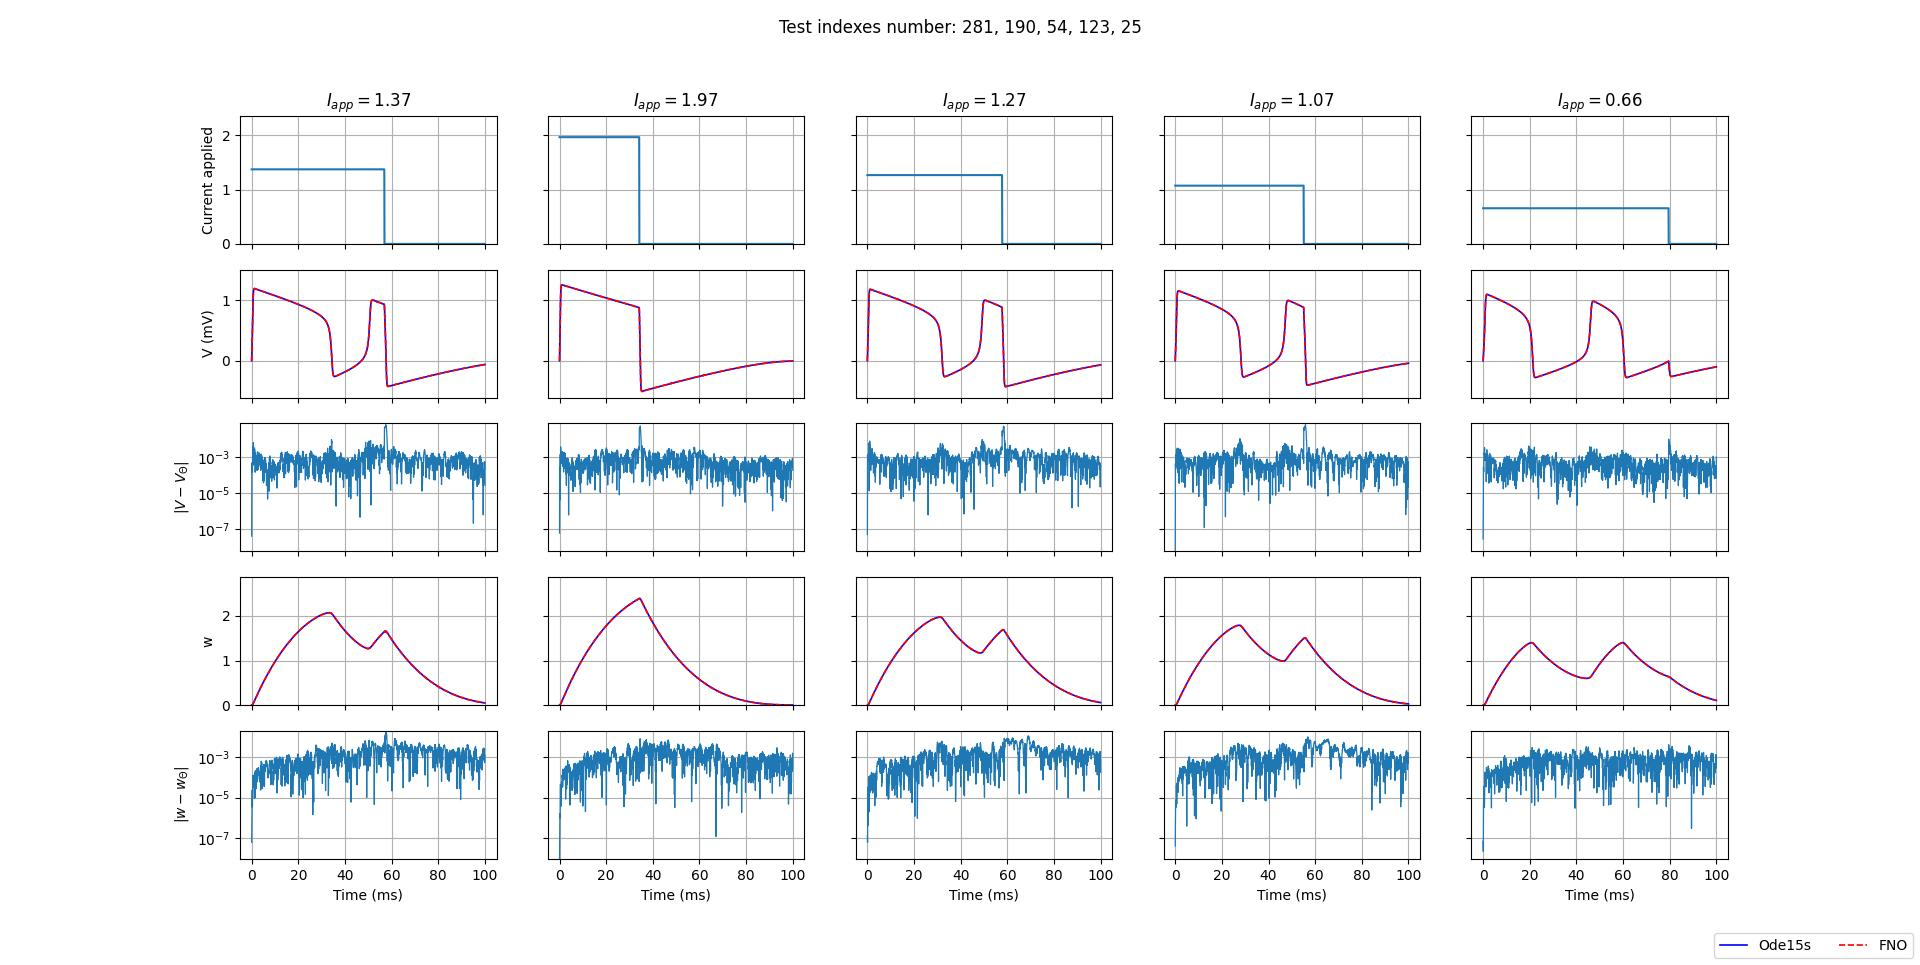
\includegraphics[width=1.8\linewidth]{images/general_error_FHN.jpg}
            \caption{Five examples for the general part of the dataset}
            \label{FHN_err_general}
        \end{subfigure}

        \begin{subfigure}{.5\textwidth}
            \centering
            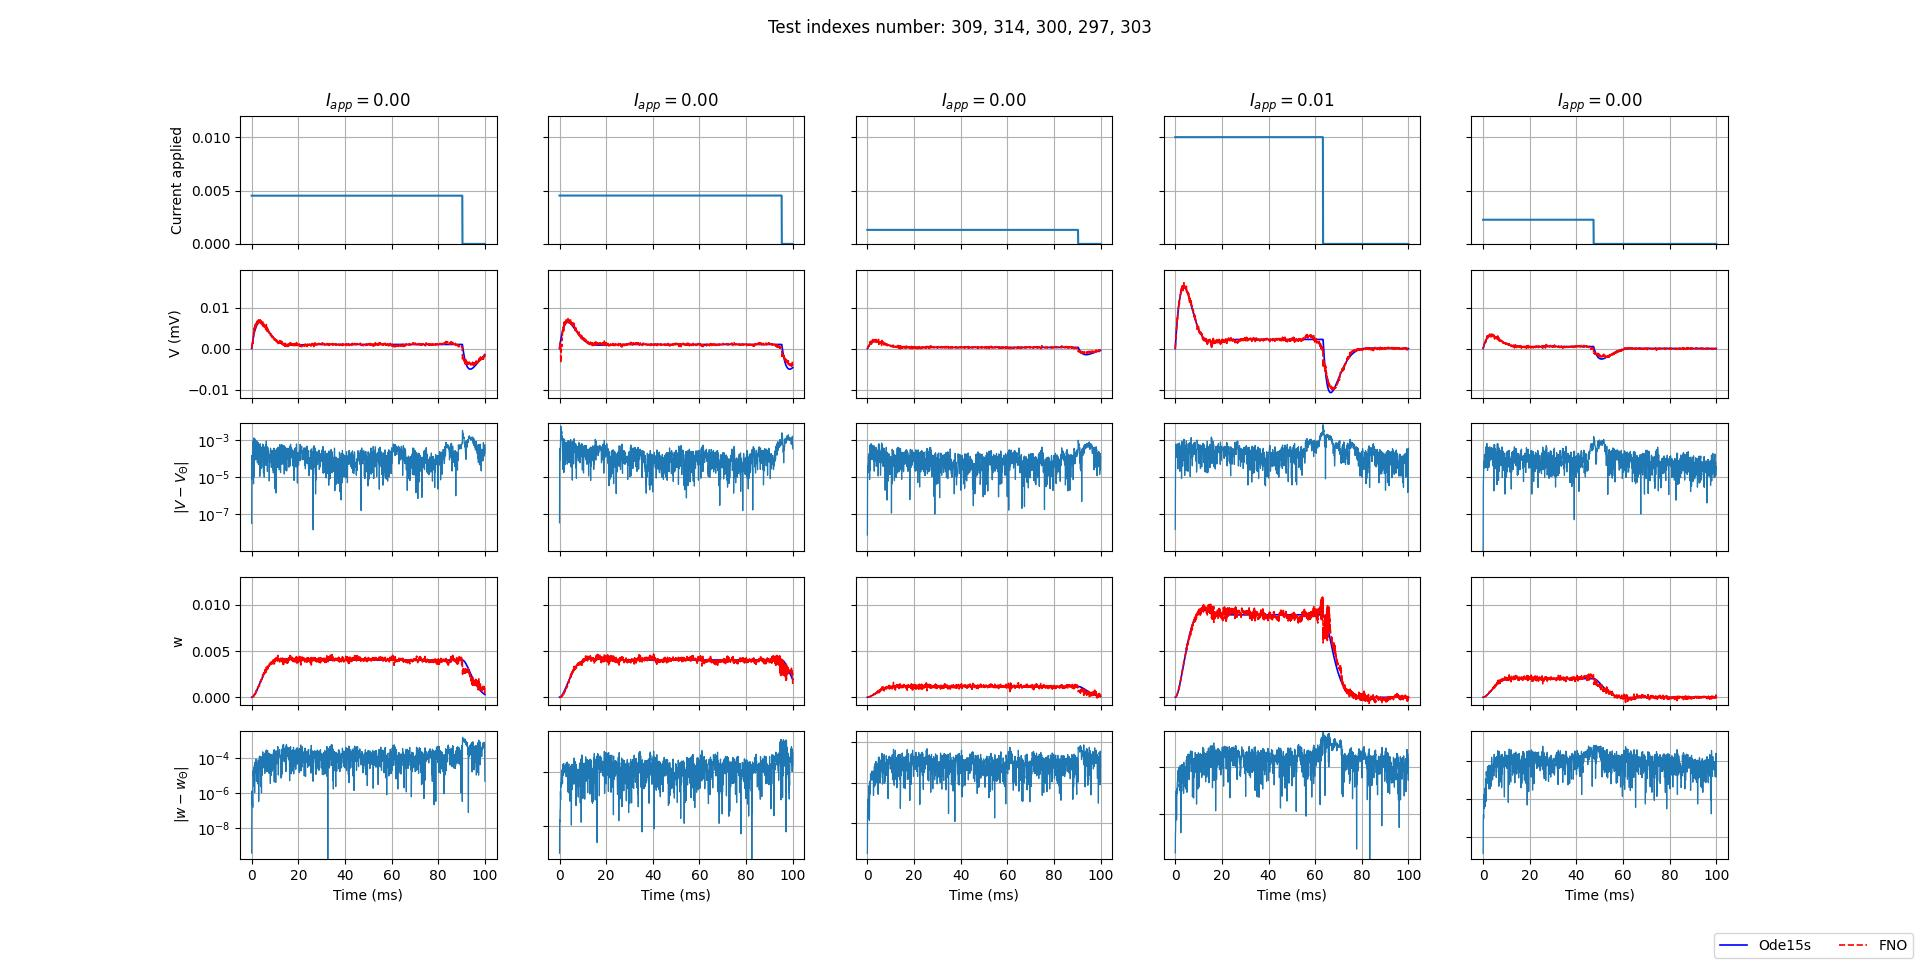
\includegraphics[width=1.8\linewidth]{images/nap_error_FHN.jpg}
            \caption{Five examples for the nap part of the dataset}
            \label{FHN_err_nap}
        \end{subfigure}

        \begin{subfigure}{.5\textwidth}
            \centering
            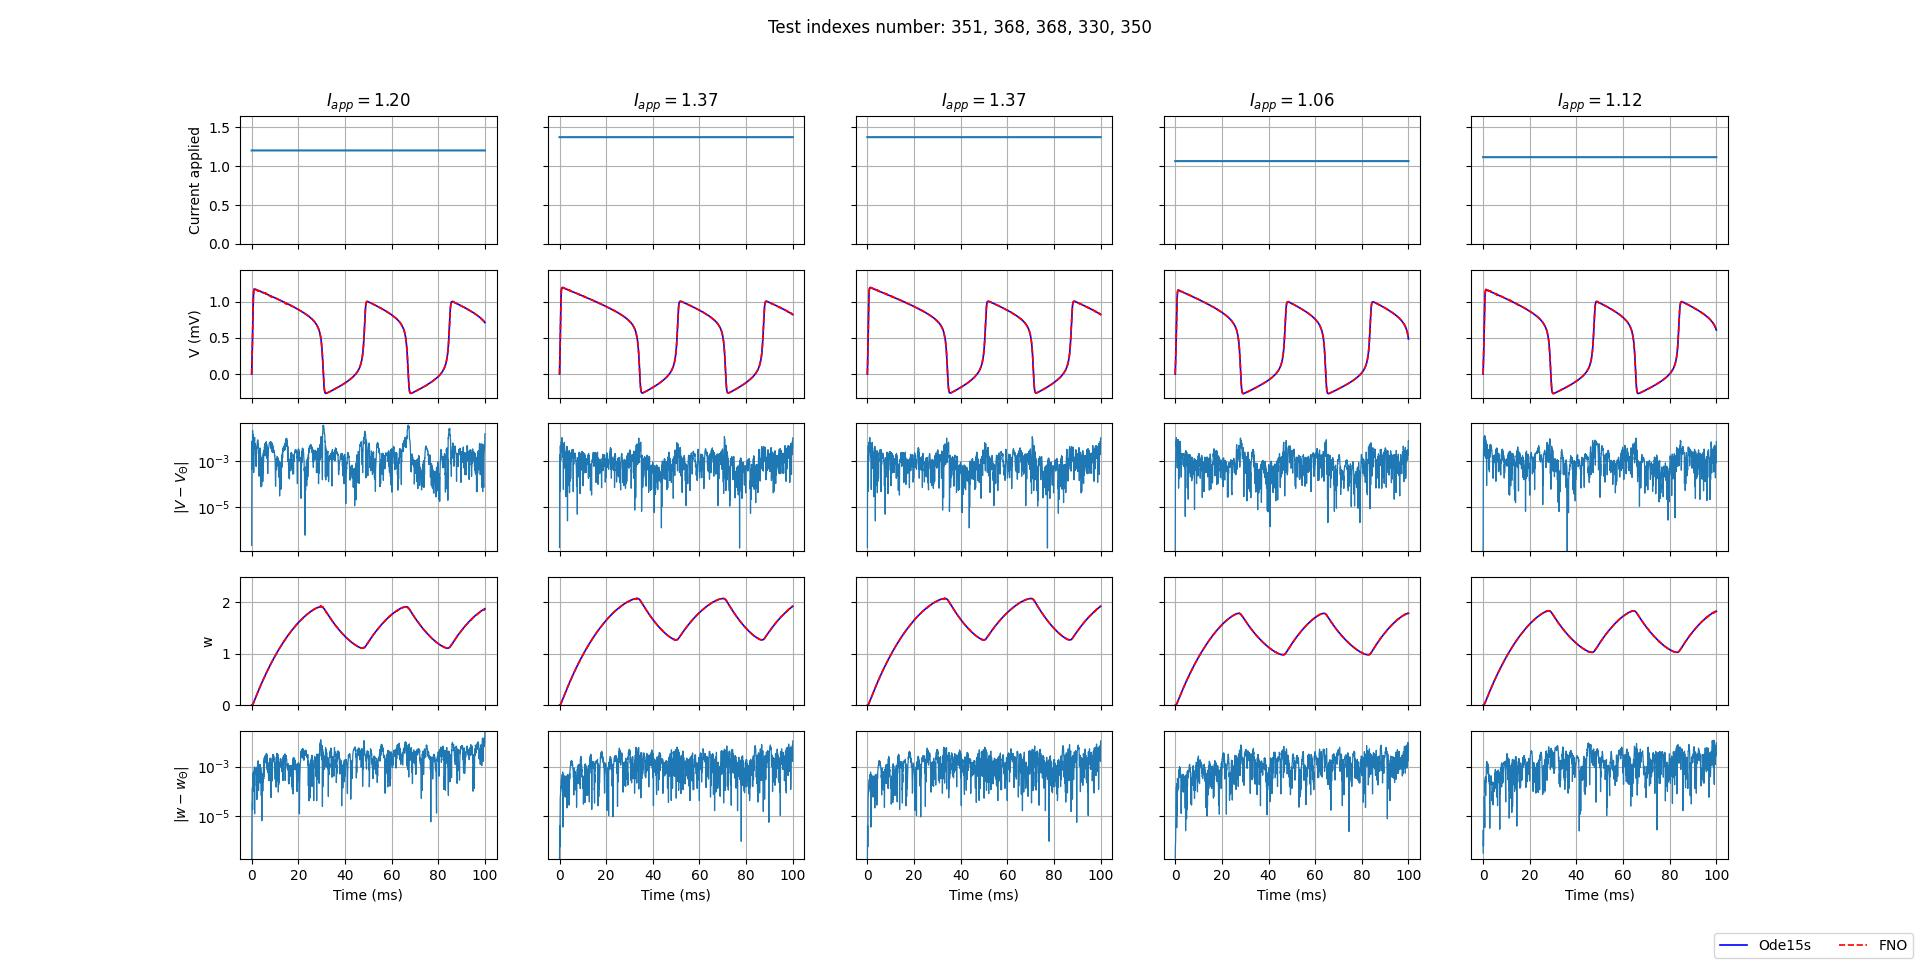
\includegraphics[width=1.8\linewidth]{images/t_f_error_FHN.jpg}
            \caption{Five examples for the $t_{fin}$ part of the dataset}
            \label{FHN_err_t_f}
        \end{subfigure}
        \caption{Each figure contains five plots, arranged in order from the top row as follows: current applied, voltage, point-wise error for the voltage, recovery variable $w$, and point-wise error for the recovery variable.}
        \label{Grafici FHN }
    \end{figure}
\end{center}



\subsection{Architecture}
\mg{Finire ray}

\section{Hodgkin-Huxley}
\begin{center}
    $\begin{cases}
            C_m\frac{dV}{dt} = -\Big(\bar{g}_{Na}m^3h(V-V_{Na}) +\bar{g}_Kn^4(V-V_K)+\bar{g}_L(V-V_L)\Big) +I_{app}, \ \  & t\in[0,T], \\[15pt]

            \frac{dm}{dt} = \alpha_m(V)(1-m)-\beta_m(V)m, \ \                                                             & t\in[0,T], \\[15pt]
            \frac{dh}{dt} = \alpha_h(V)(1-h)-\beta_h(V)h, \ \                                                             & t\in[0,T], \\[15pt]
            \frac{dn}{dt} = \alpha_n(V)(1-n)-\beta_n(V)n, \ \                                                             & t\in[0,T], \\[15pt]

            V(0) = 2.7570e-02,                                                                                                         \\[15pt]
            m(0) = 5.2934e-02,                                                                                                         \\[15pt]
            h(0) = 5.9611e-01,                                                                                                         \\[15pt]
            n(0) = 3.1768e-01.
        \end{cases}$
\end{center}
Where
\begin{multicols}{2}
    \begin{itemize}
        \item $C_m =1$
        \item $\bar{g}_{Na}=120$
        \item $\bar{g}_K =36$
        \item $\bar{g}_L =0.3$
        \item $V_{Na}=115$
        \item $V_K=-12$
        \item $V_L=10.6$
    \end{itemize}
\end{multicols}
\begin{align*}
     & \alpha_m(V)=0.1(25-V)\Big[\exp\Big(\frac{25-V}{10}\Big)\Big]^{-1}    &  & \beta_m(V)=4\exp\Big(-\frac{V}{18}\Big)                 \\
     & \alpha_h(V)=0.07\exp\Big(-\frac{V}{20}\Big)                          &  & \beta_h(V)=\Big[\exp\Big(\frac{30-V}{10}\Big)\Big]^{-1} \\
     & \alpha_n(V)=0.01(10-V)\Big[\exp\Big(\frac{10-V}{10}\Big)-1\Big]^{-1} &  & \beta_n(V)=0.125\exp\Big(-\frac{V}{80}\Big)             \\
\end{align*}

Our objective is to learn the operator

\begin{alignat*}{2}
    \Op : & \IR        &  & \rightarrow  H^1([0,T];\IR)\times H^1([0,T];\IR)\times H^1([0,T];\IR)\times H^1([0,T];\IR) \\
          & I_{app}(t) &  & \mapsto (V(t),m(t),h(t),n(t))
\end{alignat*}
\subsection{Dataset}
The dataset is formed using odes15s of matlab with $T=1$. Where we radomly pick the intenstiy of the current and the duration of the stimolus $T_{stim}$. In order to get all the imporant dynamics of the system the generation of the dataset for the training is splitted in three formed in the following way (i nomi sono quelli usati su matlab) \mg{training con il nuovo dataset con nap =  20 }\lp{Ridurre il numero di esempi per il caso del $t_0$ e metterre aggiungere i casi del $t_{fin}$}
\begin{center}
    \begin{tabular}{cccc}
        \hline
        Name       & Range of sampling for the current & Range of sampling for $T_{stim}$ & $n_{examples}$       \\
        \hline\hline
        $t_0$      & $(2,10)$                          & $(0,0)$                          & \textcolor{red}{200} \\
        General    & $(2,10)$                          & $(0.01,1)$                       & 2200                 \\
        nap        & $(1e-7,2)$                        & $(0.1,1)$                        & 300                  \\
        $i_{high}$ & $(50,200)$                        & $(0.1,1)$                        & 300                  \\
        \hline
    \end{tabular}
\end{center}
For the testing we genera 375 example where the dataset is splitted in four.
\begin{center}
    \begin{tabular}{cccc}
        \hline
        Name       & Range of sampling for the current & Range of sampling for $T_{stim}$ & $n_{examples}$      \\
        \hline\hline
        $t_0$      & $(0.1,2)$                         & $(0,0)$                          & \textcolor{red}{10} \\
        General    & $(0.1,2)$                         & $(0.01,1)$                       & 275                 \\
        nap        & $(1e-7,0.01)$                     & $(0.1,1)$                        & 30                  \\
        $i_{high}$ & $(50,200)$                        & $(0.1,1)$                        & 30                  \\
        $t_{fin}$  & $(10,30)$                         & $(1,1)$                          & 30                  \\
        \hline
    \end{tabular}
\end{center}
As before we take five examples for each part of the test dataset (General,$i_{high}$,nap,$t_fin$) and visualize the results in figure \ref{Grafici HH}.

\begin{center}
    \begin{figure*}
        \begin{subfigure}{.5\textwidth}
            \centering
            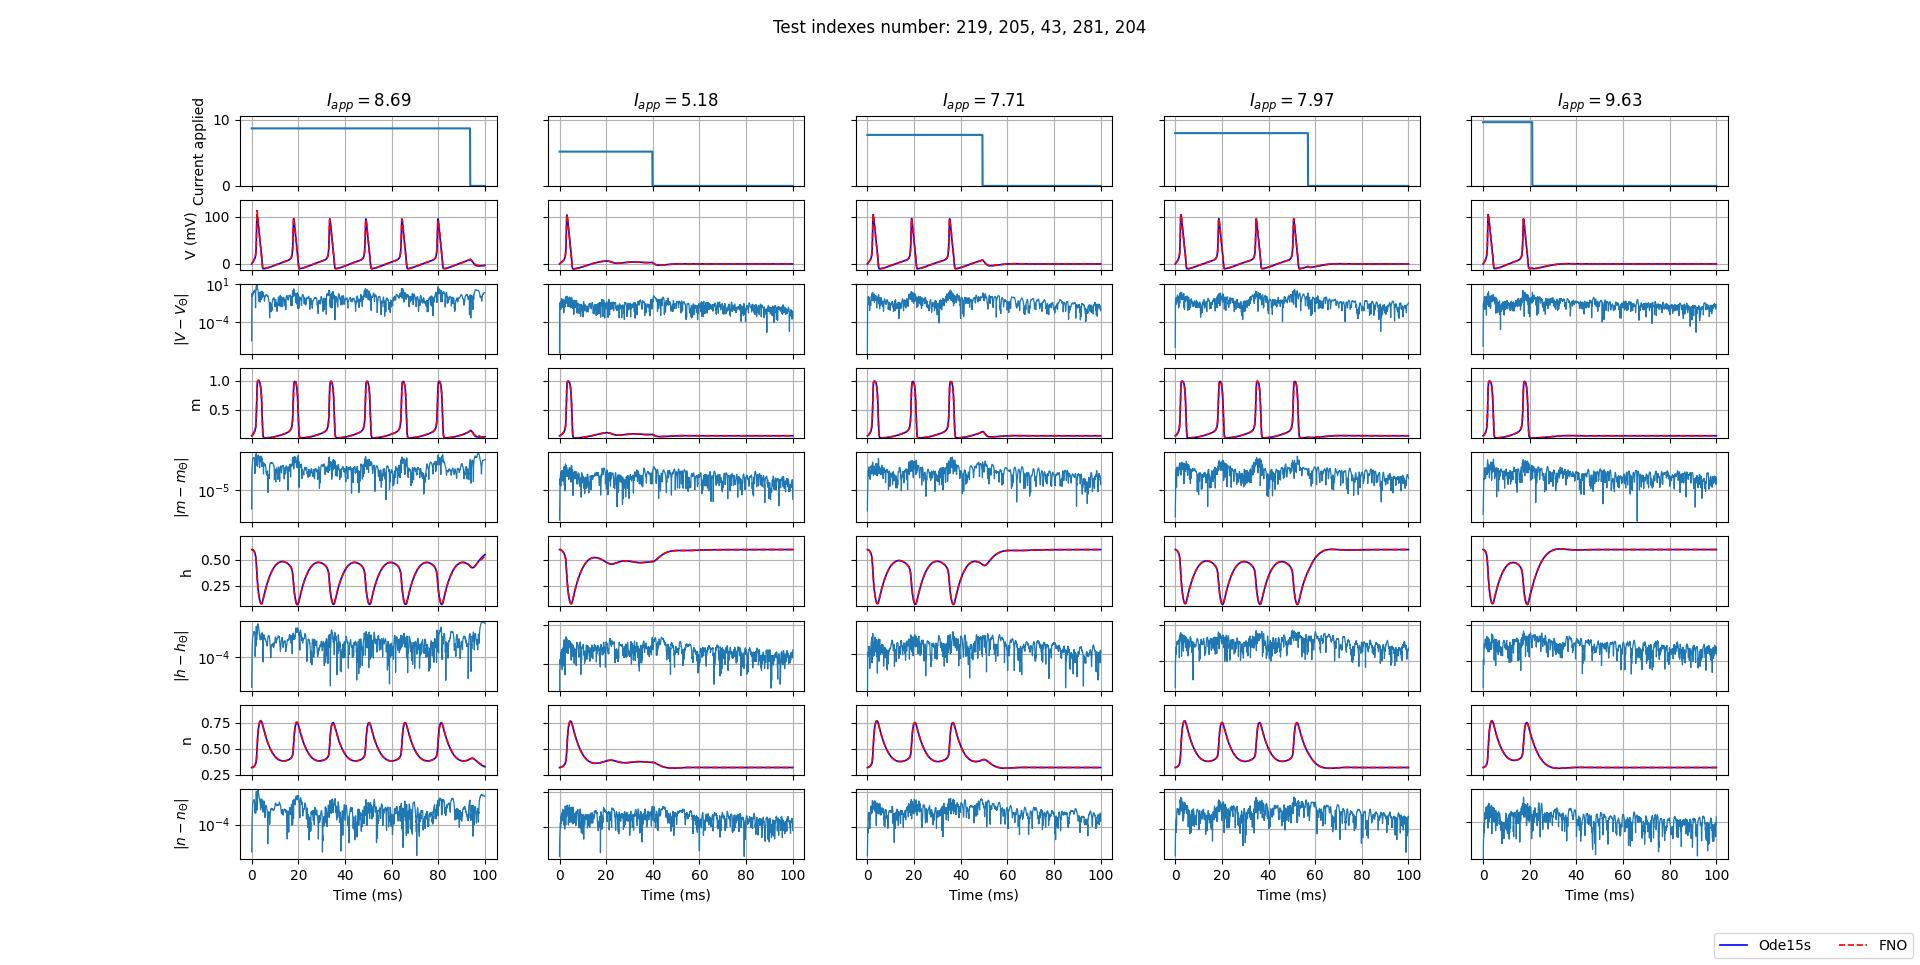
\includegraphics[width=1.8\linewidth]{images/general_error_HH.jpg}
            \caption{Five examples for the general dataset}
            \label{HH_err_general}
        \end{subfigure}

        \begin{subfigure}{.5\textwidth}
            \centering
            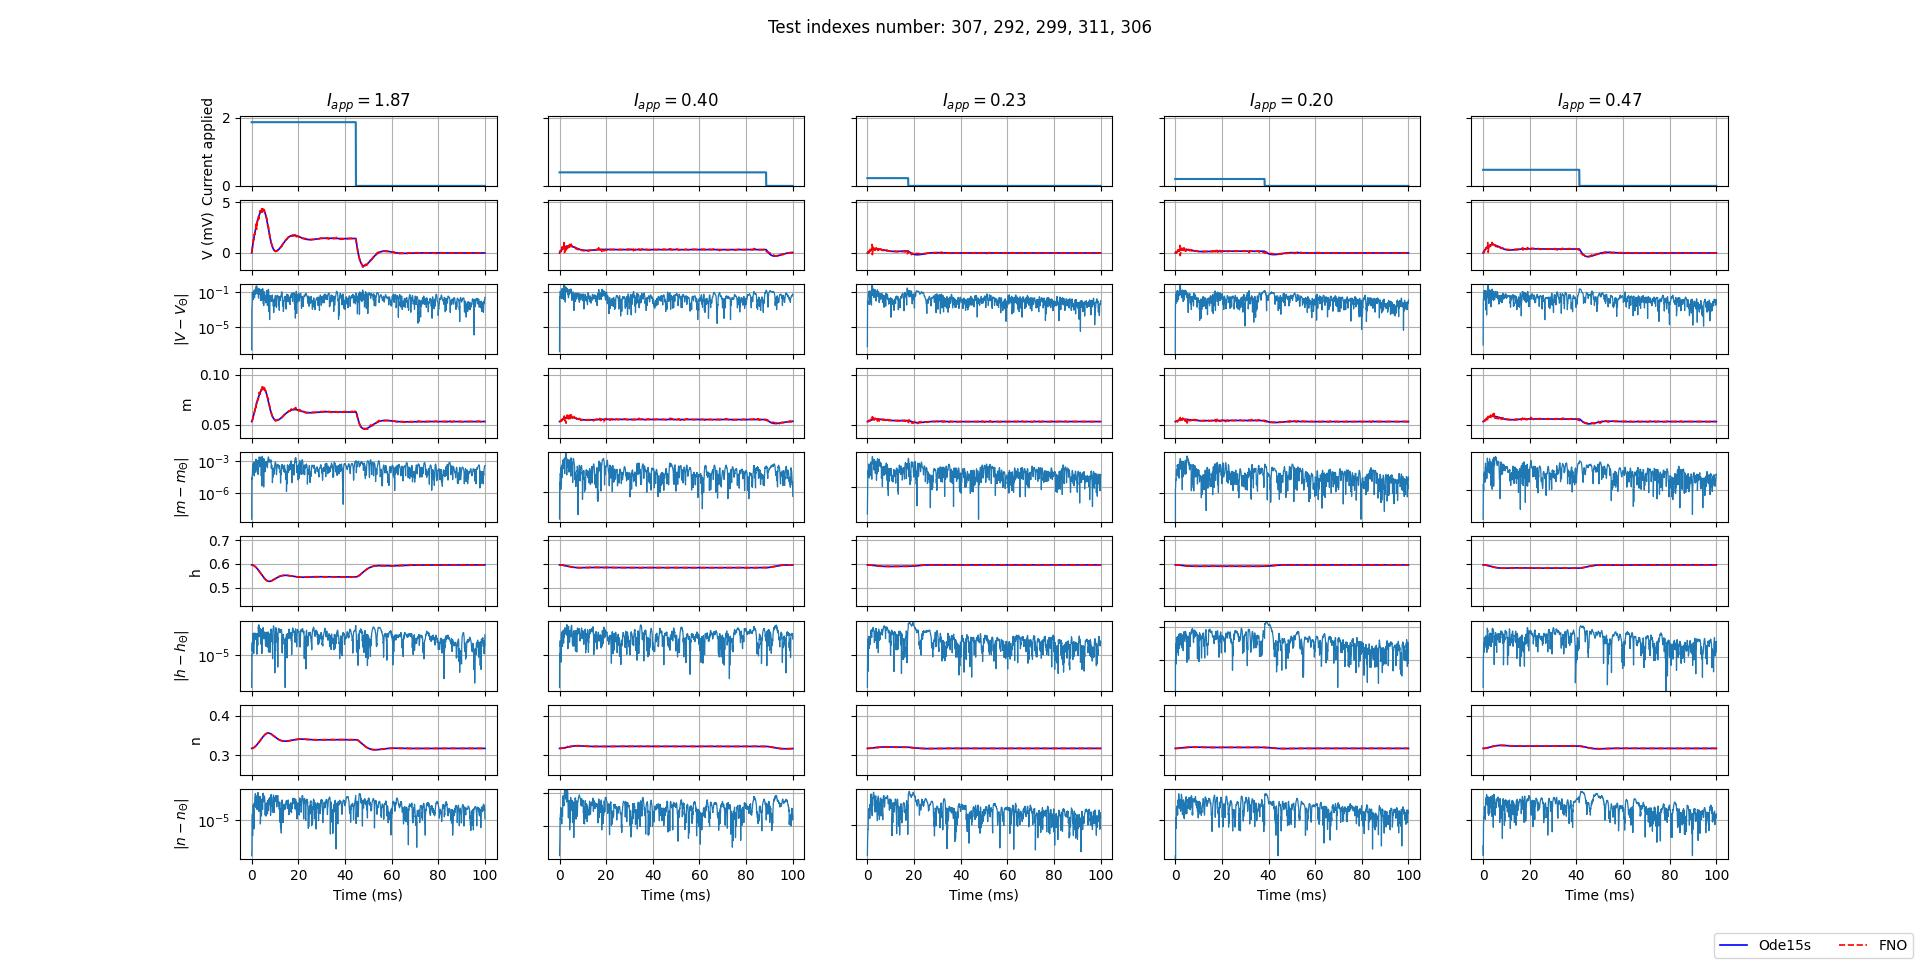
\includegraphics[width=1.8\linewidth]{images/nap_error_HH.jpg}
            \caption{Five examples for the nap dataset}
            \label{HH_err_nap}
        \end{subfigure}

        \begin{subfigure}{.5\textwidth}
            \centering
            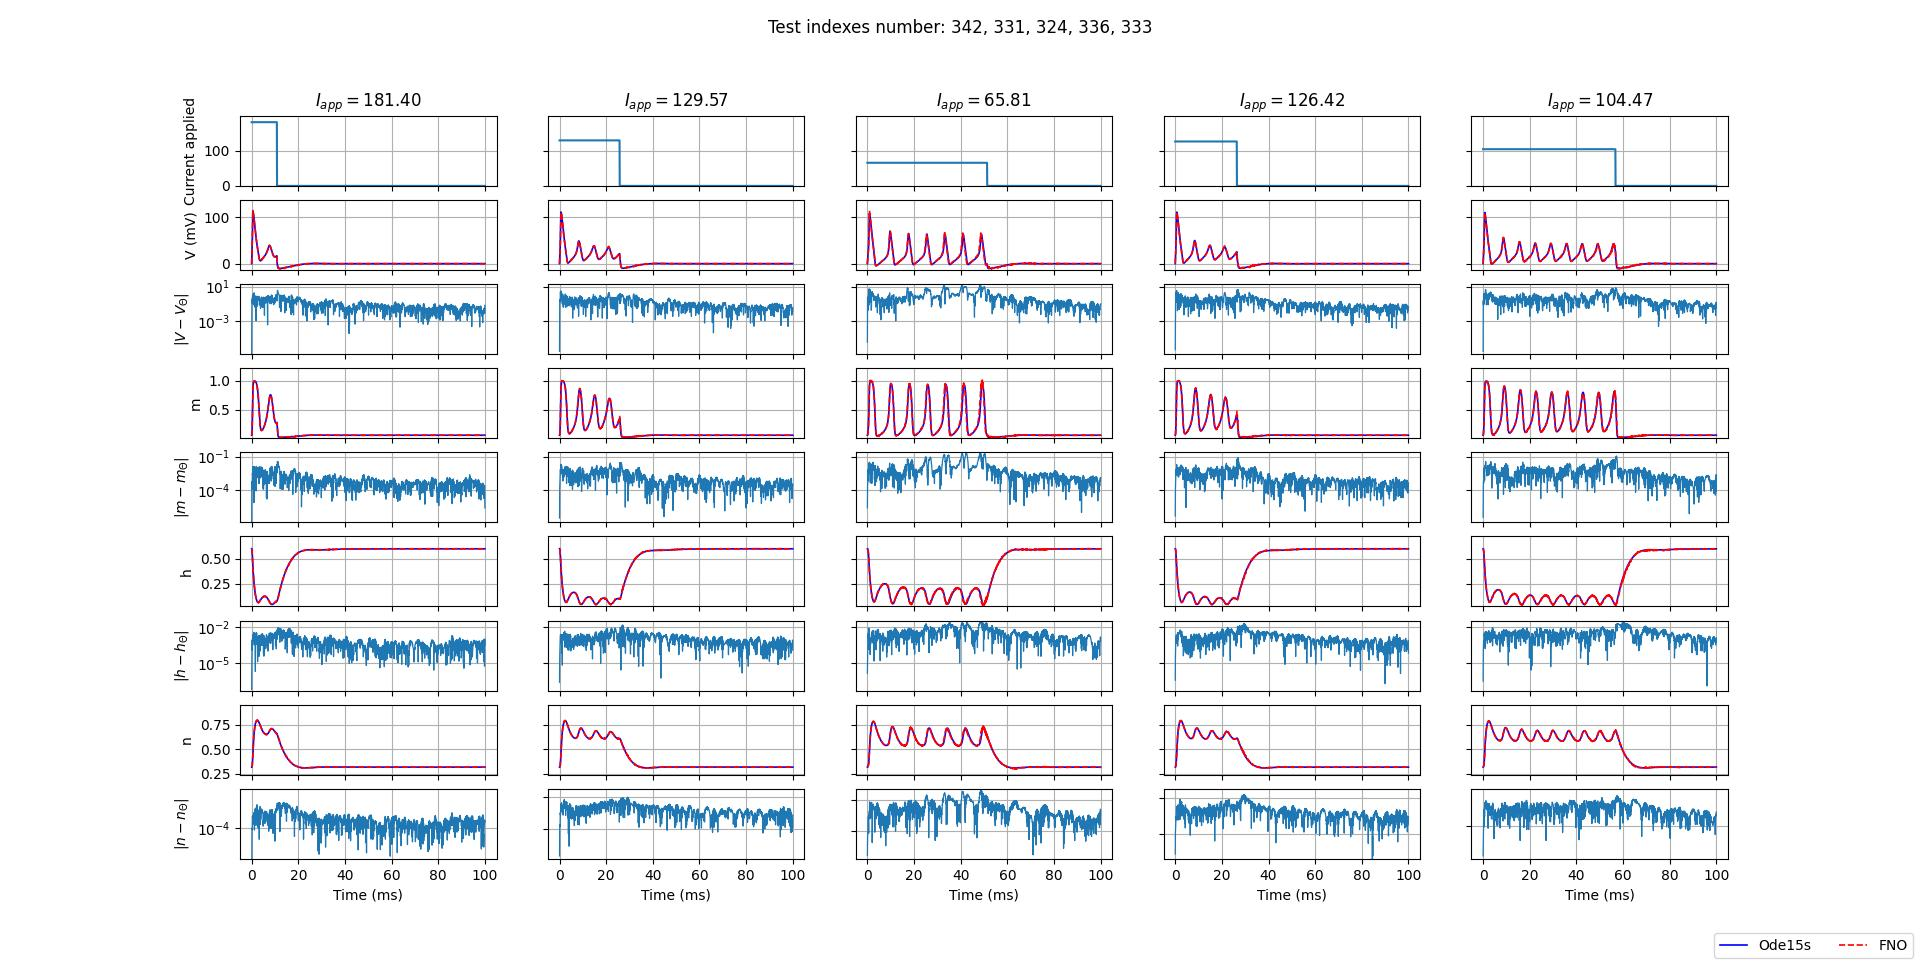
\includegraphics[width=1.8\linewidth]{images/high_i_error_HH.jpg}
            \caption{Five examples for the $i_{high}$ dataset}
            \label{HH_err_t_f}
        \end{subfigure}
    \end{figure*}
\end{center}
\newpage
\begin{figure}
    \begin{subfigure}{.5\textwidth}

        \centering
        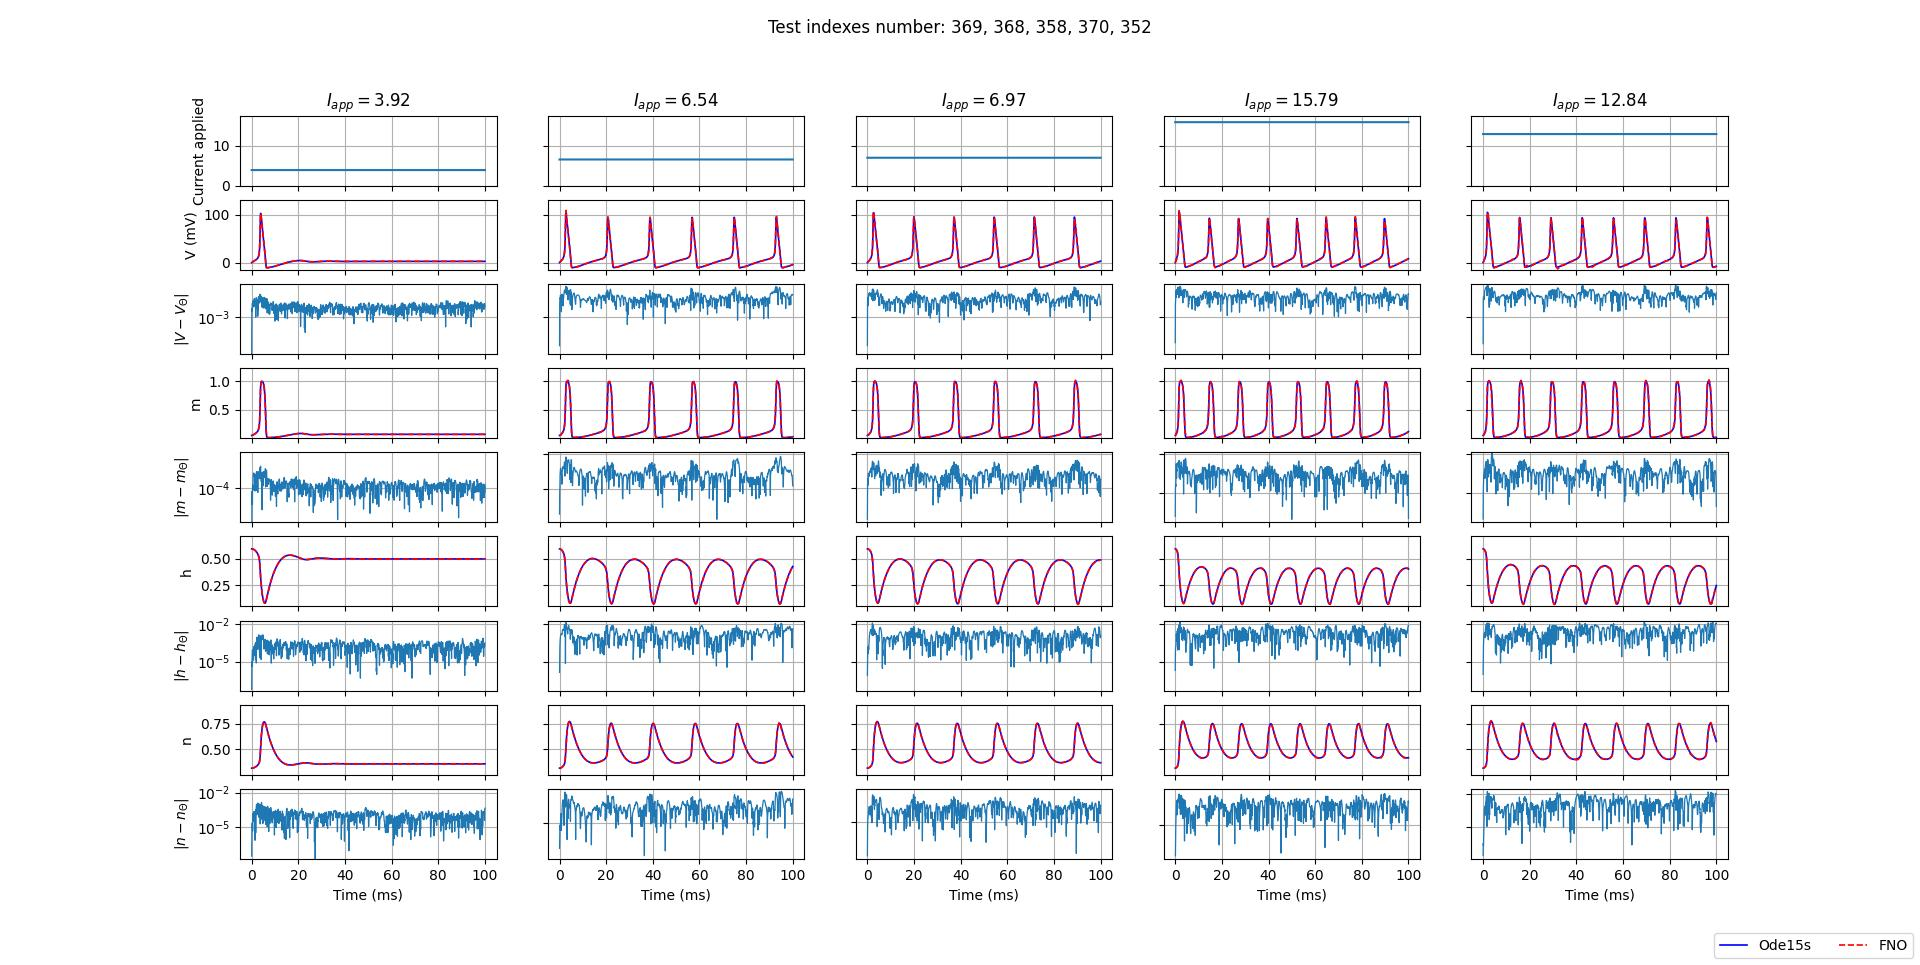
\includegraphics[width=1.8\linewidth]{images/t_f_error_HH.jpg}
        \caption{Five examples for the $t_{fin}$ dataset}
        \label{HH_err_t_f}
    \end{subfigure}
    \caption{Results obtained each of the figures has the following graph in order from the top row: current applied, Voltage, point-wise error for the Voltage,gating variable m, point-wise error for m,gating variable n,point-wise error for n,gating variable h, error for the gating variable h}
    \label{Grafici HH}
\end{figure}
\end{document}
